\begin{table}[H]
    \centering
    \begin{tabular}{|c|c|c|c|c|}
        \hline
        \multicolumn{5}{|c|}{Trees} \\
        \Xhline{3\arrayrulewidth}
        Tree & Insert $x$ & Delete $x$ & Search $x$ & Remark \\
        \Xhline{2\arrayrulewidth}
        BST & \multicolumn{3}{c|}{$O(\log n) \sim O(n)$} & Create: $O(n\log n) \sim O(n^2)$ \\
        \hline
        AVL tree & \multicolumn{3}{c|}{\multirow{4}{*}{$O(\log_m n)$}} & $F_{h + 2} - 1 \le n \le 2^h - 1$ \\
        \cline{1-1}\cline{5-5}
        B tree & \multicolumn{3}{c|}{} & $1 + 2\frac{\ceil{\frac{m}{2}}^{h - 1} - 1}{\ceil{\frac{m}{2}} - 1} \le n \le \frac{m^h - 1}{m - 1}$ \\
        \cline{1-1}\cline{5-5}
        RBT & \multicolumn{3}{c|}{} & $h \le 2\log (n + 1)$ \\
        \cline{1-1}\cline{5-5}
        Splay tree & \multicolumn{3}{c|}{} & Worst: $O(n)$, Amortized: $O(\log n)$ \\
        \hline
    \end{tabular}
\end{table}

\begin{table}[H]
    \centering
    \begin{tabular}{|c|c|c|c|c|c|}
        \hline
        \multicolumn{6}{|c|}{Priority queues} \\
        \Xhline{3\arrayrulewidth}
        Operations & Max (Min) & \makecell{Min-max \&\\Deap \&\\SMMH} & Leftist & Binomial & Fibonacci \\
        \Xhline{2\arrayrulewidth}
        Insert $x$ & $O(\log n)$ & $O(\log n)$ & $O(\log n)$ & $O(\log n), O(1)^*$ & $O(1)^*$ \\
        \hline
        Delete max & $O(\log n)$ & $O(\log n)$ & & & \\
        \hline
        Delete min & $O(n)$ & $O(\log n)$ & $O(\log n)$ & $O(\log n)$ & $O(\log n)^*$ \\
        \hline
        Delete $x$ & & & & $O(\log n)$ & $O(\log n)^*$ \\
        \hline
        Merge & $O(n)$ & & $O(\log n)$ & $O(\log n)$ & $O(1)^*$ \\
        \hline
        Decrease key & & & & $O(\log n)$ & $O(1)^*$ \\
        \hline
        Search $x$ & $O(n)$ & & & & \\
        \hline
        Find max & $O(1)$ & $O(1)$ & & & \\
        \hline
        Find min & & $O(1)$ & & $O(\log n)$ & $O(1)$ \\
        \hline
        Remark & & & \makecell{$shortest(\text{root})$\\$\le \log (n + 1) - 1$} & & \\
        \hline
    \end{tabular}
\end{table}

\begin{table}[H]
    \centering
    \begin{tabular}{|c|c|c|c|c|c|}
        \hline
        \multicolumn{6}{|c|}{Sorting algorithms} \\
        \Xhline{3\arrayrulewidth}
        \multirow{2}{*}{Method} & \multicolumn{3}{c|}{Time complexity} & \multirow{2}{*}{Space complexity} & \multirow{2}{*}{Stable} \\
        \cline{2-4}
        & Best & Worst & Average & & \\
        \Xhline{2\arrayrulewidth}
        Insertion & $O(n)$ & \multicolumn{2}{c|}{$O(n^2)$} & $O(1)$ & $\surd$ \\
        \hline
        Selection & \multicolumn{3}{c|}{$O(n^2)$} & $O(1)$ & $\texttimes$ \\
        \hline
        Bubble & $O(n)$ & \multicolumn{2}{c|}{$O(n^2)$} & $O(1)$ & $\surd$ \\
        \hline
        Shell & $O(n^{1.5})$ & \multicolumn{2}{c|}{$O(n^2)$} & $O(1)$ & $\texttimes$ \\
        \hline
        Quick & $O(n\log n)$ & $O(n^2)$ & $O(n\log n)$ & $O(\log n) \sim O(n)$ & $\texttimes$ \\
        \hline
        Merge & \multicolumn{3}{c|}{$O(n\log n)$} & $O(n)$ & $\surd$ \\
        \hline
        Heap & \multicolumn{3}{c|}{$O(n\log n)$} & $O(1)$ & $\texttimes$ \\
        \hline
        LSD Radix & \multicolumn{3}{c|}{$O(n \times k)$} & $O(n + k)$ & $\surd$ \\
        \hline
        Bucket/MSD Radix & $O(n)$ & $O(n^2)$ & $O(n + k)$ & $O(n \times k)$ & $\surd$ \\
        \hline
        Counting & \multicolumn{4}{c|}{$O(n + k)$} & $\surd$ \\
        \hline
    \end{tabular}
\end{table}

\begin{table}[H]
    \centering
    \begin{tabular}{|c|c|c|}
        \hline
        \multicolumn{3}{|c|}{Dynamic Programming algorithms} \\
        \Xhline{3\arrayrulewidth}
        Problem & Time complexity & Space complexity \\
        \Xhline{2\arrayrulewidth}
        Making change & $O(kn)$ & $O(n)$ \\
        \hline
        Fractional Knapsack problem & $\Theta(n\log n)$ & $O(n)$ \\
        \hline
        0/1 Knapsack problem (DP) & $O(n2^{\log W})$ & $O(n2^{\log W})$ \\
        \hline
        0/1 Knapsack problem (Branch-and-Bound) & $O(2^n)$ & \\
        \hline
        Longest Common Subsequence (LCS) & $O(mn)$ & $O(mn)$ \\
        \hline
        Longest Increasing Subsequence (LIS) & $O(n^2)$ & $O(n^2)$ \\
        \hline
        Longest Common Substring & $O(mn)$ & $O(mn)$ \\
        \hline
        Minimum Edit Distance & $O(mn)$ & $O(mn)$ \\
        \hline
        Matrix-chain Multiplication & $O(n^3)$ & $O(n^2)$ \\
        \hline
        Traveling Salesperson problem & $\Theta(n^22^n)$ & $O(n2^n)$ \\
        \hline
        Optimal Binary Search Tree (OBST) & $\Theta(n^3)$ & $\Theta(n^2)$ \\
        \hline
    \end{tabular}
\end{table}

\begin{table}[H]
    \centering
    \begin{tabular}{|c|c|c|}
        \hline
        \multicolumn{3}{|c|}{Graph algorithms} \\
        \Xhline{3\arrayrulewidth}
        Problem & Time complexity & Remark \\
        \Xhline{2\arrayrulewidth}
        Depth-First Search (DFS) & $O(|\V| + |\E|)$ & \\
        \hline
        Kosaraju's & $O(|\V| + |\E|)$ & \\
        \hline
        Kruskal's & $O(|\E|\log |\V|)$ & \\
        \hline
        Prim's (Adjacency matrix) & $O(|\V|^2)$ & \\
        \hline
        Prim's (Adjacency list) & $O(|\V||\E|)$ & \\
        \hline
        Prim's (Min-Heap, Adjacency list) & $O(|\E|\log |\V|)$ & \\
        \hline
        Prim's (Fibonacci heap, Adjacency list) & $O(|\E| + |\V|\log |\V|)$ & \\
        \hline
        Sollin's (Borůvka's) & $O(|\E|\log |\V|)$ & \\
        \hline
        Dijkstra's (Min-heap) & $\Theta((|\E| + |\V|)\log |\V|)$ & \multirow{2}{*}{\makecell{Greedy, no negative\\edges or cycles}} \\
        \cline{1-2}
        Dijkstra's (Fibonacci-heap) & $\Theta(|\E| + |\V|\log|\V|)$ &  \\
        \hline
        Bellman-Ford & $O(|\V||\E|)$ & DP \\
        \hline
        Floyd-Warshall & $\Theta(|\V|^3)$ & DP, no negative cycles \\
        \hline
        Johnson's & $\Theta(|\V||\E| + |\V|^2\log |\V|)$ & No negative cycles \\
        \hline
        Ford-Fulkerson & $O(|\E||f^*|)$ & Greedy,$f^*$為最大流 \\
        \hline
        Edmond-Karp & $O(|\V||\E|^2)$ & \\
        \hline
        Push-relabel & $O(|\V|^2|\E|)$ & \\
        \hline
    \end{tabular}
\end{table}

\begin{itemize}
    \item Matrix-chain Multiplication:\begin{equation}
        m[i, j] = \begin{cases}
            0 &, i = j \\
            \min_{i \le k \le j - 1}\{m[i, k] + m[k + 1, j] + p_{i - 1}p_kp_j\} &, i < j
        \end{cases}
    \end{equation} 
    \item Optimal Binary Search Tree (OBST):\begin{equation}
        \begin{aligned}
            e[i, j] & = \begin{cases}
                q_{i - 1} &, j = i - 1 \\
                \min_{i \le r \le j}\{e[i, r - 1] + e[r + 1, j] + w[i, j]\} &, i \le j
            \end{cases} \\
            w[i, j] & = w[i, j - 1] + p_j + q_j
        \end{aligned}
    \end{equation}
    \item Minimum vertex cover (tree):\begin{equation}
        \begin{aligned}
            V(v) = \min \{& 1 + \Sum\{V(c), \ \forall c \in v.child\}, \\
            & \len\{v.child\} + \Sum\{V(g), \ \forall c \in v.child \ \forall g \in c.child\}
        \}   
        \end{aligned}
    \end{equation} First part: root is in the cover; second part: root is NOT in the cover.
    \item Max-cut: \begin{itemize}
        \item NPC。
        \item 若所有邊權重皆負,則可乘上$-1$,變為Min-cut。
        \item 若為平面圖,可轉換為Chinese Postman Problem(若為無向圖,即Euler circuit,若為有向圖,則為NPC)。
    \end{itemize}
    \item 如果可以證明\textbf{lower bound} of \textbf{worst case} of NPC problems is polynomial,則$P=NP$。
    \begin{figure}[H]
        \centering
        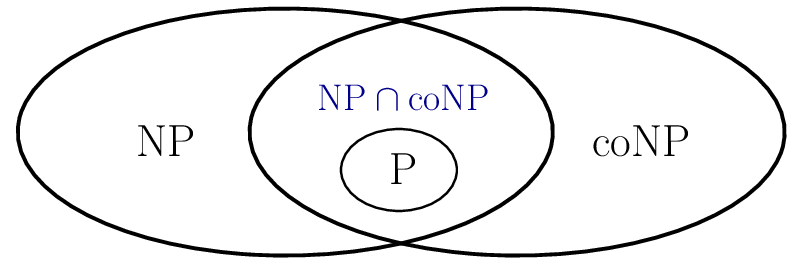
\includegraphics[scale=0.4]{img/np-conp.png}
        \caption{Relationship between NP and CO-NP.}
        \label{img:np-conp}
    \end{figure}
    \item Permutation:
    \begin{algorithm}[H]
        \begin{algorithmic}[1]
            \Function{Perm}{$list, i, n$}
                \If {$i == n$}
                    \State \Call{Print}{$list$}
                \Else
                    \For {$j$ := $i$ to $n$}
                        \State \Call{Swap}{$list$, $i$, $j$}
                        \State \Call{Perm}{$list$, $i + 1$, $n$}
                        \State \Call{Swap}{$list$, $i$, $j$}
                    \EndFor
                \EndIf
            \EndFunction
        \end{algorithmic}
    \end{algorithm}
    \item 節點數:\begin{equation}
        \begin{aligned}
            n & = (\sum_{i = 1}^{\deg}i \times n_i) + 1 \\
            n_0 & = n_2 + 1 \ \text{(二叉樹)}
        \end{aligned}
    \end{equation}
    \item \quad\quad
    \begin{algorithm}[H]
        \begin{algorithmic}[1]
            \Function{CreateMinHeap}{Tree $s$, size $n$}
                \For {$i$ := $n / 2$ to 1} \Comment{Start from parent of the last node.}
                    \State $tmp$ := $s[i]$
                    \State $j$ := $2 \times i$ \Comment{Left child of $i$.}
                    \While {$j \le n$} \Comment{There is a child.}
                        \If {$j < n$} \Comment{Right child exists.}
                            \If {$s[j] > s[j + 1]$} \Comment{Choose the smaller child.}
                                \State $j$ := $j + 1$
                            \EndIf
                        \EndIf
                        \If {$tmp \le s[j]$}
                            \State Break.
                        \Else \Comment{Percolate one level.}
                            \State $s[j / 2]$ := $s[j]$
                            \State $j$ := $j \times 2$
                        \EndIf
                    \EndWhile
                    \State $s[j / 2]$ := $tmp$
                \EndFor
            \EndFunction
        \end{algorithmic}
    \end{algorithm}
    \item 尋找articulation point:若root有$\ge 2$子節點,則root為articulation point;
    $\exists$ 非root節點$u$,若$\exists \ v$為$u$子節點,且$low(v) \ge dfn(u)$,則$u$為articulation point。
    \begin{figure}[H]
        \centering
        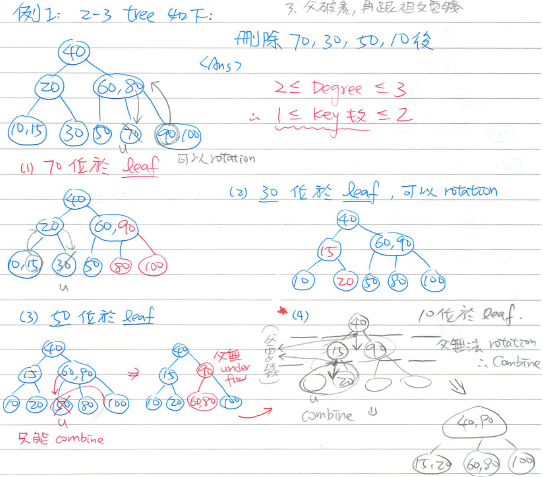
\includegraphics[scale=0.55]{summary/btree_del.png}
        \caption{Example of B-tree deletion.}
        \label{img:np-conp}
    \end{figure}
    \item (\textbf{FALSE}) For two functions $f(n)$ and $g(n)$, either $f(n) = O(g(n))$ or $f(n) = \Omega((f(n))$.
    Counterexample:\begin{equation}
        \begin{aligned}
            f(n) & = \begin{cases}
                1, \ \text{if} \ n = 2k \\
                0, \ \text{if} \ n = 2k + 1
            \end{cases} \\
            g(n) & = \begin{cases}
                0, \ \text{if} \ n = 2k \\
                1, \ \text{if} \ n = 2k + 1
            \end{cases} 
        \end{aligned}
    \end{equation}
    \item For any uniform cost RAM program $T(n) = \Omega(S(n))$, where $S(n)$ is the space an algorithm uses for an input of size $n$.
    \item The capacity of each edge of a flow network can be floating-point, and it can be solved by linear programming.
    \item A flow network of multiple sources can be reduced to a single source.
    \item (\textbf{FALSE}) The value of any flow of a flow network is bounded by the capacity of only at most $O(n)$ cuts.
    \item 2-coloring: $O(n^2)$, 3-coloring, 4-coloring: superpolynomial.
    \item Weighted-union heuristic: Append the \textbf{smaller} list onto the \textbf{longer} list, with ties broken arbitrarily.
    \item $n! \neq \Theta(n^n)$.
    \item A DAG with $n$ vertices can \textbf{NOT} have more than $\binom{n}{2}$ edges.
    \item Longest palindrome subsequence: \begin{equation}
        \begin{aligned}
            & L(i, j) = \begin{cases}
                0 &, i = j + 1 \\
                1 &, i = j \\
                L(i + 1, j - 1) + 2 &, i < j \land s[i] = s[j] \\
                \max(L(i + 1, j), L(j, j - 1)) &, \text{otherwise}
            \end{cases} \\
            & \text{where} \ L[1 \cdots n][1 \cdots n], s[1 \cdots n]
        \end{aligned}
    \end{equation}
    \item Minimum triangulation: \begin{equation}
        c(i, j) = \begin{cases}
            0 &, j < i + 2 \\
            \min_{i < k < j}\{c(i, k) + c(k, j) + dist(i, j) + dis(j, k) + dist(k, j)\} &, \text{otherwise}
        \end{cases}
    \end{equation} \begin{lstlisting}[caption={Minimum triangulation.}, captionpos=b]
        double triangulation(Point P[], int n) {
            if (n < 3)
                return 0;
            
            double c[n][n];
            for (int gap = 0, gap < n; gap++) {
                for(int i = 0, j = gap; j < n; i++, j++) {
                    if (j < i + 2)
                        c[i][j] = 0.0;
                    else {
                        c[i][j] = MAX;
                        for (int k = i + 1; k < j; k++) {
                            double val = c[i][k] + c[k][j] + wt(P, i, j, k);
                            if (c[i][j] > val)
                                c[i][j] = val;
                        }
                    }
                }
            }

            return c[0][n - 1];
        }
    \end{lstlisting}
    \item Sort $n$ integers ranged from $0$ to $n^2 - 1$: 將$n$個整數表示成\textbf{n進位}數,每個數由$2$-digit表示,範圍$0$到$n - 1$,再用radix sort對$2$-digit排序,共兩次。
    \item If max frequency is $\le 2$ times of min frequency, Huffman code is \textbf{NOT} always better than an ordinary fixed-length code.
    \item Amortized analysis與average-case analysis無關。
    \item (\textbf{FALSE}) \textbf{If} a graph has a unique MST then, for every cut of the graph, there is a \textbf{unique light edge} crossing the cut.
    \item (\textbf{TRUE}) A graph has a unique MST \textbf{if}, for every cut of the graph, there is a \textbf{unique light edge} crossing the cut.
    \item The worst-case running time and expected running time are equal to within \textbf{constant} factors for any randomized algorithm.
    \item Selection problem: $T(n) = T(\frac{n}{5}) + T(\frac{3n}{4}) + O(n)$
    \item Given an \textbf{undirected} graph and a positive integer $k$, is there a path of length $\le k$, which each edge has weight $1$ and each vertex is visited \textbf{exactly} once: P, solved by Floyd-Warshall algorithm.
    \item Given an \textbf{undirected} graph and a positive integer $k$, is there a path of length $\ge k$, which each edge has weight $1$ and each vertex is visited $\le$ once: NPC.
    \item A flow network of multiple sources can be reduced to a single source.
    \item Subset sum: $s(i, j)$: sum $j$ can be found in $\{a_1, \ \cdots, a_i\}$ \begin{equation}
        s(i, j) = \begin{cases}
            0 &, i = 0 \\
            1 &, j = 0 \\
            s(i - 1, j) \lor s(i - 1, j - v_i) &, j \ge v_i
        \end{cases}
    \end{equation} result is $s(m, n)$.
    \item Hanoi tower iterative version: Check if the \textbf{input number} $n$ is even or odd. \\ 
    If $n$ is even, \begin{equation}
        \begin{cases}
            A \leftrightarrow C \\
            A \leftrightarrow B \\
            C \leftrightarrow B
        \end{cases} 
    \end{equation} If $n$ is odd, \begin{equation}
        \begin{cases}
            A \leftrightarrow B \\
            A \leftrightarrow C \\
            B \leftrightarrow C
        \end{cases} 
    \end{equation}
    \item Fibonacci search: \begin{lstlisting}[caption={Fibonacci search.}, captionpos=b, language=Python]
        def fibSearch(arr, data):
            max = len(arr) - 1
            y = getY(fib, max + 1) # Find the largest index, which its value is smaller than data.
            m = max - fib[y] 
            x = y - 1
            i = x
            if arr[i] < data: # Check at first.
                i += m
            while fib[x] > 0:
                if arr[i] < data:
                    x -= 1
                    i += fib[x]
                elif arr[i] > data:
                    x -= 1
                    i -= fib[x]
                else:
                    return i
            return -1
    \end{lstlisting}
    \item Box stacking: \begin{enumerate}
        \item Generate all $3$ rotations of all boxes. We consider width as always smaller than or equal to depth.
        \item Sort the above generated $3n$ boxes in \textbf{decreasing} order of \textbf{base area}.
        \item $msh(i)$: Max possible stack height with box $i$ at top of stack. \begin{equation}
            \begin{aligned}
                msh(i) = \{& \max \{msh(j)\} + height(i)\}, \\ 
                & \forall j < i \land width(j) > width(i) \land depth(j) > depth(i)
            \end{aligned}
        \end{equation} result is \begin{equation}
            \max_{0 < i < n}\{msh(i)\}
        \end{equation}
    \end{enumerate}
    \item Building bridge: \begin{enumerate}
        \item Sort the north-south pairs on the basis of \textbf{increasing} order of \textbf{south} x-coordinates.
        \item Find \textbf{LIS} of north x-coordinates.
    \end{enumerate}
    \item Optimal strategy: $f(i, j)$: max value the user can collect from $i$-th coin to $j$-th coin.\begin{equation}
        f(i, j) = \begin{cases}
            v_i &, j = i \\
            \max\{v_i, v_j\} &, j = i + 1 \\
            \begin{aligned}
                \max\{& v_i + \min\{f(i + 2, j), f(i + 1, j -1)\}, \\
                & v_j + \min\{f(i + 1, j -1), f(i, j - 2)\}\}
            \end{aligned} &, \text{otherwise}
        \end{cases}
    \end{equation}
    \item (TIOJ-1097) Find the largest square submatrix with all 0s in a 0/1 matrix: $dp(i, j)$: max square submatrix in $i \times j$ left upper submatrix. \begin{equation}
        dp(i, j) = \min\{dp(i − 1, j − 1), dp(i, j − 1), dp(i − 1,j)\} + 1
    \end{equation} 
    \item (UVA-10934) Dropping water balloons ($k$ balloons and height $n$): $dp(i, j)$: max height $i$ balloons can be dropped $j$ times. \begin{equation}
        dp(i, j) = \begin{cases}
            dp(i, j - 1) + dp(i - 1, j - 1) + 1 &, arr(i, j) = 1 \\
            0 &, arr(i, j) = 0
        \end{cases}
    \end{equation} result is \begin{equation}
        \min_{j} \{dp(k, j) \ge n\}
    \end{equation}
    \item (TIOJ-1471) Skyline: $dp(i, j)$: walk $i$ distance and height is $j$. \begin{equation}
        \begin{cases}
            dp(i, j) & = dp(i - 1, j - 1) + sum(j) \\
            sum(j) & = sum(j) -dp(i - j, j) + dp(i, j)
        \end{cases}
    \end{equation} result is \begin{equation}
        \sum_{j}dp(n, j)
    \end{equation}
    \item Largest rectangle in histogram: \begin{itemize}
        \item If the new element is higher than stack top element, push it; otherwise, pop and calculate the area until the new element is higher than stack top element.
        \item Maximal rectangle: Similarly, for each column, the count of $1$ of each row, can be seen as the element.
    \end{itemize}
    \item \quad\quad \begin{itemize}
        \item AVL trees are ideal for sorting items of an \textbf{ordered dictionary}.
        \item Different number binary trees of height $h$: \begin{equation}
            H_n = \begin{cases}
                2H_{n - 1} \times \sum\limits_{i = 0}^{h - 2}H_i + H_{i - 1}^2 &, h \ge 2\\
                H_0 = 1, H_1 = 3 
            \end{cases}
        \end{equation}
    \end{itemize}
\end{itemize}

\pagebreak
